\subsection{Photo-multipliers surface coating}

The PMTs used in the LTCC are the photonis are the Photonis XP4500B \cite{Photonis:2007ta}.
Their borosilicate windows can be used to detect wavelengths as low as approximately
$300$ nm. However the Cherenkov light is inversely proportional to the wavelegth, see eq.~\ref{eq:cerenkov},
the $C_4F_{10}$ gas is transparent down to wavelengths of $180$ nm, and the mirrors and WCs reflectivities is non zero
even for wavelengths below $200$ nm: the limiting factor of enhanced QE in the UV region
is the transparency of the window material of the PMTs. UV-glass windows can detect photons down to
250 nm, and only quartz windows can efficiently detect light down to 180 nm. While quartz windows maximize the UV-sensitivity
of the PMT, and therefore the Cerenkov detector performance, they are difficult and expensive to produce.

A wavelength shifter (WLS) deposited on the face of a borosilicate or UV glass
PMT provides an effective alternative to boost the efficiency of a \u{C}erenkov
detector by converting UV photons with a wavelength below $300$ nm into two
isotropically emitted photons with longer wavelengths.



\begin{figure}
	\centering
	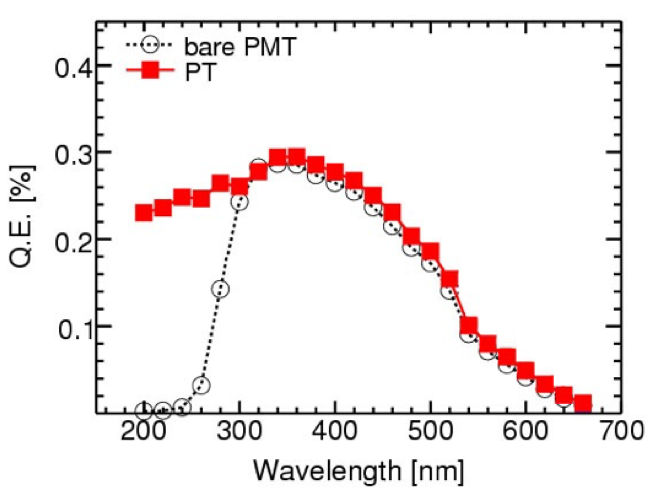
\includegraphics[width=1.0\columnwidth,keepaspectratio]{img/pmtQuantumEfficiencyGain.png}
	\caption{Average number of reflections calculated from simulations studies.}
	\label{fig:pmtQuantumEfficiencyGain}
\end{figure}

\begin{figure}
	\centering
	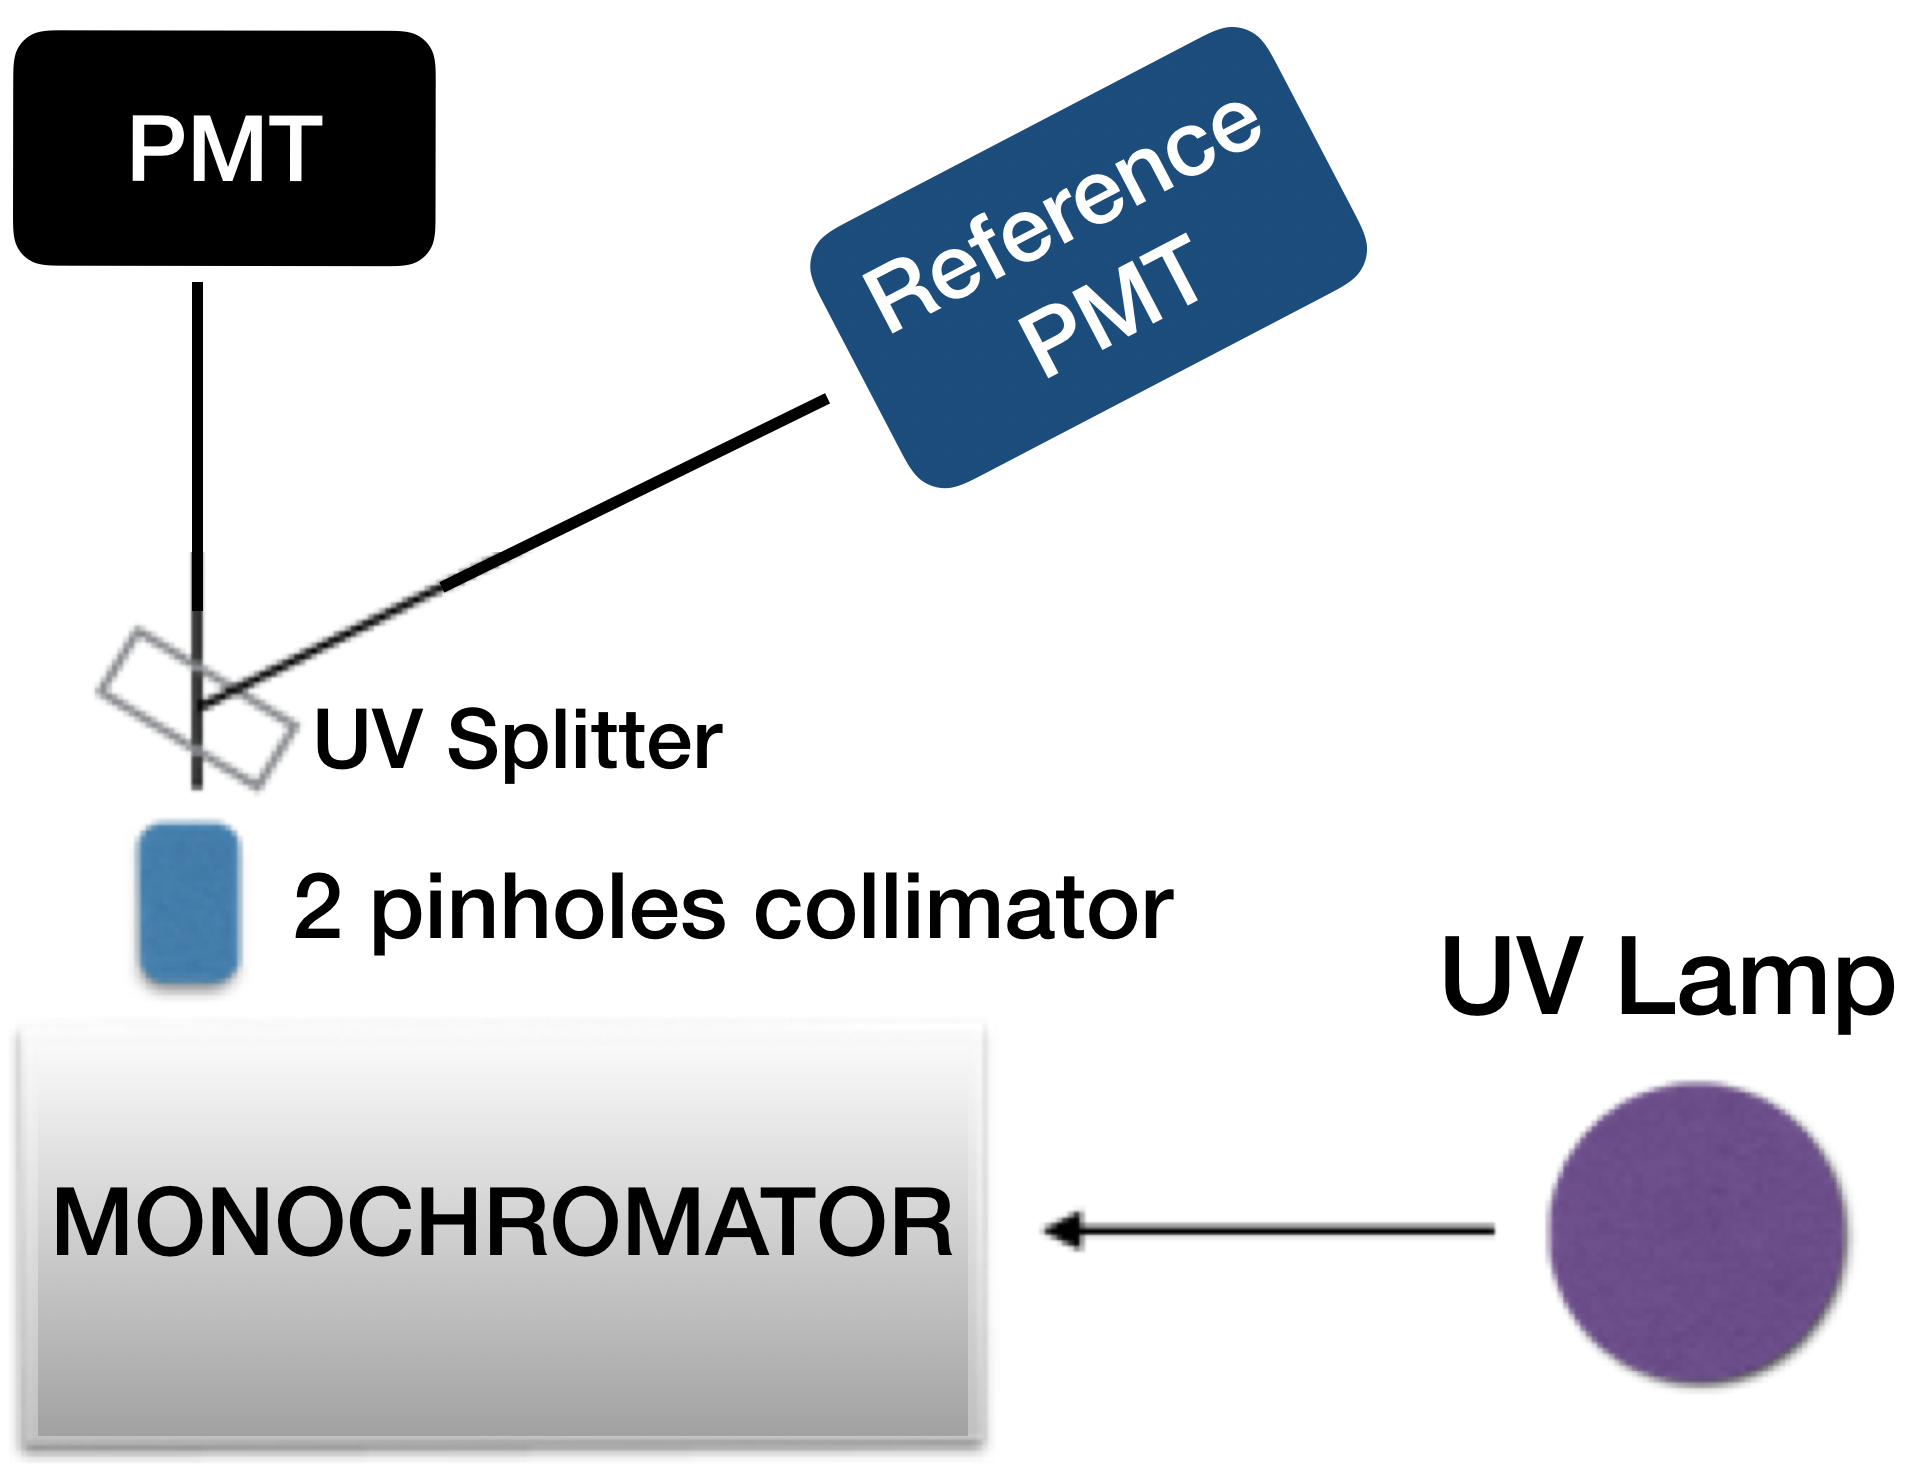
\includegraphics[width=1.0\columnwidth,keepaspectratio]{img/pmtTestingSetup.png}
	\caption{Average number of reflections calculated from simulations studies.}
	\label{fig:pmtTestingSetup}
\end{figure}



